\chapter{Drones}
\label{ch:identificador}

\section{DLV-1}

Possui uma capacidade de 2.5 kg de carga, podendo decolar com até 12.5 kg podendo percorrer 3km de ida e volta.

\begin{figure}[!ht]
    \centering
    \caption{Drone DLV-1 Drop Flash.}
    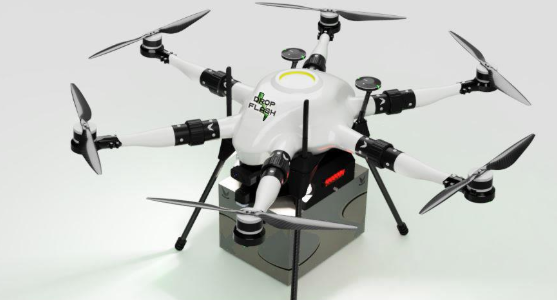
\includegraphics[width=0.6\textwidth]{figuras/DLV1.png}
    \label{fig:DLV1}\\
    \small Fonte: \url{https://www.speedbird.aero}
\end{figure}

O DLV-1 é interessante para entregas mais rápidas e leves, como documentos e artigos de farmácia, que necessitam de um tempo menor de entrega por conta de sua possível urgência\cite{Speed2024}.

\section{DLV-2}

Possui uma capacidade de 6 kg de carga e pode decolar com 25 kg de carga com 8km de ida e volta.

\begin{figure}[!ht]
    \centering
    \caption{Drone DLV-2 Drop Flash.}
    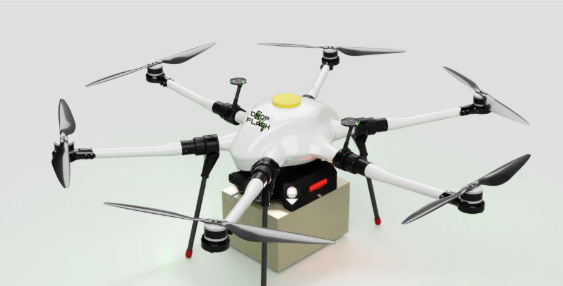
\includegraphics[width=0.6\textwidth]{figuras/Dlv 2.png}
    \label{fig:DLV2}\\
    \small Fonte: \url{https://www.speedbird.aero}
\end{figure}

O DLV-2 será utilizado para entregas de maior peso, interessante para compras no mercado ou um pedido para mais pessoas em um restaurante\cite{Speed2024}.

\section{DLV-4}

Possui uma capacidade de carga de até 5 kg, com peso máximo de decolagem dem25 kg, porém o diferencial do DLV-4 é a distância que pode percorrer, que é de até 40km de ida e volta.

\begin{figure}[!ht]
    \centering
    \caption{Drone DLV-4 Drop Flash.}
    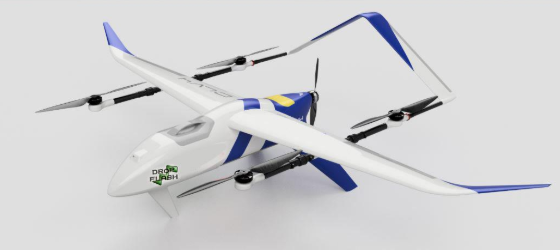
\includegraphics[width=0.6\textwidth]{figuras/dlv 4.png}
    \label{fig:DLV2}\\
    \small Fonte: \url{https://www.speedbird.aero}
\end{figure}


O DLV-4 entrega uma proposta diferente dos demais, pois tem a capacidade de realizar viagens mais longas, portanto se um cliente mora no interior ou afastado de um estabelecimento de seu interesse, é possível realizar pedidos de cidades e bairros vizinhos\cite{Speed2024}.

\section{Tecnologia utilizada nas entregas}

Os drones terão uma tecnologia que iça e baixa as cargas por meio de um cabo de aço, agilizando o procedimento de entrega. Dessa forma não existe a necessidade do drone descer até o solo para realizar a entrega, assim facilitando e a mantendo mais seguro esse procedimento\cite{Wing2024}.

\begin{figure}[!ht]
    \centering
    \caption{Exemplo de uma entrega através do cabo de aço..}
    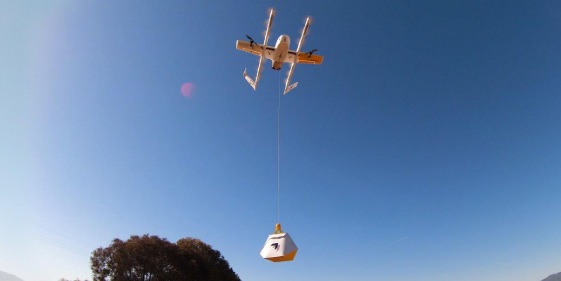
\includegraphics[width=0.6\linewidth]{figuras/tec utlzd.png}
    \label{fig:DLV2}\\
    \small Fonte: \url{https://wing.com/how-it-works/}
\end{figure}



O cabo de aço utilizado será de 3,18 mm de diâmetro com comprimento de 30 metros, que soma em 900 gramas o peso de carga do drone. O cabo em questão é forte o suficiente para suportar o peso e fino o suficiente para não sobrecarregar a carga.

\section{Pontos de decolagem e pouso}

Para cada região cadastrada existirá uma base para pouso, decolagem e manutenção dos drones. No total serão 9 bases e cada base terá 20 DLV-1, 20 DLV-2 e 10 DLV-4\cite{Speed2024}.

\begin{figure} [!ht]
    \centering
    \caption{Ilustração de um ponto de pouso e decolagem de drones da Drop Flash.}
    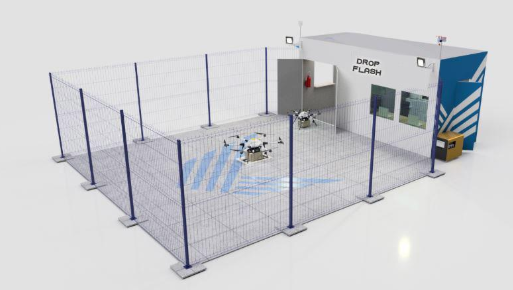
\includegraphics[width=0.6\linewidth]{figuras/p dec e po.png}
    \label{fig:enter-label}\\
    \small Fonte: \url{https://www.speedbird.aero}
\end{figure}